In this chapter, we outline and discuss the design of the project, and our 
implementation of salient components. 
We first begin with a brief overview of our core requirements and justify certain design choices.  
Next, we discuss how we approach testing -- a crucial process in the 
verification of our software components. This is followed by a section discussing the design 
choices we make for our benchmarks (Section \ref{design:bench}). After this, 
we elaborate on the general approach we take in implementing the protocols described in 
the literature. Finally, we will elaborate on the design of important components 
and their implementation.

Here, we include the components associated with each compiler for easy reference:
% General design philosphy behind each component: when we use tratis and when we use structs

\begin{enumerate}
  \item CDS94 Compiler
  \begin{itemize}
    \item Schnorr's Protocol     
    \item Shamir's Secret Sharing 
    \item CDS94 Compiler 
  \end{itemize}
  \item Stacking Sigmas Compiler
  \begin{itemize}
    \item Schnorr's Protocol 
    \item Partially-Binding Vector Commitment scheme: Q-Binding of half-bindings 
    \item Self-Stacking Compiler
  \end{itemize}
\end{enumerate}

\section{Overview}\label{design:overview}
In this section, we 
elaborate on the core requirements that influence the design choices of 
every component, discuss our choice of programming language and justify 
our choice of libraries 
that we use throughout various components of the project. 
\subsection{Core Requirements}
In the design of each component, we consider the following 
three core requirements: \emph{correctness}, \emph{generality}, and 
\emph{usability}. 

\paragraph{Correctness.} Unsurprisingly, correctness has the highest priority, 
as we want to ensure that we are accurately comparing 
the performance of the compilers. In Section \ref{design:testing}, 
we discuss how we test our compilers to ensure correctness. 

\paragraph{Generality.} This requirement is concerned with how easy it is for 
future developers to use our interfaces\footnote{Rust has different 
terminology for interfaces called "traits". While traits and classic interfaces are not 
exactly the same, they share many commonalities. For the sake of simplicity, we will 
substitute terms in Rust associated with traits with those associated with classic 
interfaces. Where this is not possible, we will explicitly use Rust terminology and 
explain the difference.}
 and components for their own work. 
One of the motivations for this project is to lay the foundations for 
future researchers to conveniently compare their own implementations 
of existing or new compilers to ours. Additionally, this will also help 
developers to easily build on our work in the future. 
With this in mind, it is important that our code is easily extensible and 
has components (which may be shared) that are modular. Thus, we have 
organised our source code such that each component is an individual
library and can be selectively chosen. This is coupled with interfaces 
designed to be as general as possible, allowing
developers to choose which components they want to use, and 
which to implement themselves. 

\paragraph{Usability.} We strive to make our compilers easy to use, understand, 
and maintain using thorough documentation and convenient 
methods to easily use the components. In the following sections, we
discuss how we attempt to achieve this in each component. 

\subsection{Programming Language}
Our choice of programming language is Rust: a modern 
language that is designed with a focus on safety and reliability.
It promises memory safety, by using an ownership and borrowing
system unique to Rust, and it is a strongly typed language which 
helps to identify errors at compile-time. This helps to prevent errors such 
as integer overflows and null pointer references. Furthermore, 
Rust is known for its high performance and speed \cite{rust-book} and 
has functional programming features such as pattern matching and 
closures. These features make Rust a good choice for our project,
particularly because many of the components we are implementing are 
defined mathematically which lend themselves well to functional 
programming. Meanwhile, robustness and speed are highly ideal properties
in any system, especially one that relies on cryptographic protocols.

Additionally, Hall-Andersen's \cite{MHAStackSig}
Stacking Sigmas compiler is also implemented in the language. This makes 
Rust a natural choice for our project, it allows us to easily compare 
our implementation to Hall-Andersen's. Rust has other useful benefits 
that pertain to more specific components of our project, such as 
testing; we highlight these in their respective sections.

\subsection{Libraries}\label{sec:libraries}
Throughout this project, a number of notable libraries are repeatedly 
used across different components. The few that we would like to highlight 
are:
\begin{enumerate}
  \item \texttt{curve25519-dalek} \cite{curve25519-dalek}: a Rust library that 
  provides group operations on the Ristretto group \cite{ristretto_web}. In many 
  of our protocols, a prime order group is required; we use this library as 
  the underlying prime order group in the concrete implementations of 
  our project. We choose the Ristretto group because it is a prime order 
  group constructed from a non-prime-order Edwards curve \cite{Edwards2007}
  (a family of elliptic curves), which is known for both security and speed. 
  At the same time, the Ristretto group does not suffer from the same issues as 
  other modern elliptic curve implementations that do not provide a prime-order group\footnote{
    Modern elliptic curve implementations usually provide a group of order $h \cdot q$, where 
    $h$ is a small cofactor (4 or 8), and $q$ is a large prime number. When using these 
    implementations for protocols that require a prime order group, the abstraction from 
    a non-prime order group to a prime order group is often handled by developers up the stack 
    (by users of the library). This means that they are not as familiar with the underlying 
      implementation, and may introduce vulnerabilities due to subtle design complications.
  }. 
  
  \item \texttt{rand\_chacha} \cite{rand-chacha}: a random number generator (RNG) that uses the 
  "ChaCha20" stream cipher \cite{bernstein2008chacha}. We use this to create RNGs 
  that are needed for our protocols. Notably, we chose this library 
  specifically because it also provides seedable RNGs, 
  which is useful for testing. 
  \item \texttt{group} \cite{group}: a library that provides general interfaces for 
  groups and fields. In the pursuit to make our components as general as 
  possible, we make use of the interfaces in this library to define the 
  kind of groups and fields that are accepted by our interfaces. When users 
  develop their own concrete implementation of our interfaces, they can 
  choose to use any group or field that implements the interfaces in this 
  library and are not restricted to the concrete implementations that we 
  provide. 
\end{enumerate} 


\section{Testing}\label{design:testing}
As mentioned in Project Management (Chapter \ref{ch:project-management}), we use Test-Driven Development to 
ensure correctness. By writing tests before features, we encourage focus on the 
requirements of our software and ensure that we design our components to target 
these requirements. Once these tests are written, we have an efficient workflow to 
consistently ensure our software is correct, even as we add new features. This improves
development speed and reduces the time needed to identify and fix bugs.

In addition, we perform extensive static analysis to complement testing and improve 
debugging. To support static analysis, we 
intentionally design our components and interfaces to reflect their 
mathematical definitions in the literature. A good example of this is our implementation of q-bindings and half-bindings
(Section \ref{design:qbinding}). Doing this allows us to easily verify that our implementations
adhere to their mathematical definitions as closely as possible, increasing the chances of 
identifying an issue if there is one.

\paragraph{Unit \& Integration Testing.}
We use the built-in testing framework in Rust to test our components. This framework allows us to write unit 
tests within the same source code file as our implementation, and conveniently run them within our 
IDE (VSCode) which consequently speeds up development. We also write integration tests with 
the same framework, except that they are often located in a separate file to emphasise that they are testing 
multiple components as these components have to be explicitly imported into the scope of the this testing module. 

\paragraph{Code Coverage.} To complement testing, we use code coverage reports to ensure that we are testing 
as much of our code as possible. Code coverage is a way to track and determine which sections of code (e.g. 
functions, branches, lines etc.) are executed. This is useful for us as it highlights sections of code that 
are neglected by our existing tests and ensures that we cover important test cases. We use the 
\texttt{cargo-llvm-cov} \cite{cargo-llvm-cov} tool to carry out code coverage analysis. 
This tool is a wrapper around the Rust compiler's in-built code coverage tool, 
providing a convenient way to generate code coverage reports as they integrate directly 
with our testing suite. 

\subsection{Extracting Requirements \& Writing Tests}
Throughout this project, the requirements of our software components are mostly derived 
from the literature with the exception of our benchmarks. Therefore, our testing 
strategy is centered around testing these requirements against our implementation. Of 
course, additional unit tests are written to test the correctness of specific functions
as well, but we will not discuss these in detail. 

Extracting these requirements is a manual process that requires a thorough 
understanding of the literature. Our approach begins with reading the literature and
writing down the requirements explicitly. This is a tedious process,
but it is necessary to ensure that we have a complete understanding of the protocols
and what is required of them. We then translate these requirements into tests. 
\begin{enumerate}
  \item Usually, the first step is to complete a function for setting up mock data 
  that is likely to be used in the tests. We design this function to take in a set of 
  parameters and returns a set of mock data. These can then be separately called in 
  each test, with parameters, to generate data specific for that test. 
  \item Next, we write the content of the tests themselves. Because we are desining our 
  components to model the mathematical definitions of the protocols, we can often easily 
  determine the exact methods to call. Often, a 
  challenge in TDD is not knowing what functions are available to test because they 
  are not yet implemented. However, this is not a problem in this project as we have 
  the definitions in the literature to refer to. There are two main kinds of tests 
  that we write:
  \begin{itemize}
    \item \textbf{Positive Tests:} These are tests that ensure the implementation
    works as expected. 
    \item \textbf{Negative Tests:} These are tests that ensure the implementation
    fails as expected.
  \end{itemize}
  \item Following this, we proceed to implement our components. This often starts with 
  the interfaces (if any), and then to any classes that are required. 
  \item Finally, we run the tests to ensure that they pass. If they do not, we 
  investigate and either fix the implementation or the tests.
\end{enumerate}

In Appendix \ref{code:cds-tests}, we provide an example of our tests with those 
for the CDS94 compiler. Often the first tests that are written target the main 
requirements that we glean from the literature. As development progresses, we 
continue to write tests or extend existing ones to ensure that we are testing 
comprehensively. 


\section{Benchmarks}\label{design:bench}
In our benchmarks, we are concerned with measuring the growth of certain 
metrics when the number of clauses in the disjunction increases. Suppose 
we have a disjunctive zero-knowledge proof $\Pi = (A, Z, \phi)$, then 
the metrics we are concerned with are as follows:
\begin{enumerate}
  \item \textbf{Communication Complexity:} 
  size of communication between the prover and verifier (in bytes). This is 
  the size of the messages $a \leftarrow A$, $z \leftarrow Z$, and $c \leftarrow \{0,1\}^\kappa$.
  \item \textbf{Prover Computation Time:}
  time taken for the prover to run the algorithms $A$ and $Z$ 
  \item \textbf{Verifier Computation Time:}
  time taken for the verifier to run the algorithm $\phi$.
\end{enumerate}

Crucially, we are also interested in learning the \textbf{total computational time} of 
the compiled proof, which we can easily computed by summing the prover and verifier 
running times. 

We target these three metrics as they are the main properties 
that are measurable and are used for evaluating the performance of the compiled 
proofs. Other properties such as security limitations (e.g. the requirement for a
trusted setup) are not measurable, and thus are not considered in our benchmarks.

The range we use for our clauses is $(2, 2^2, \ldots, 2^{13})$; this means that 
at each step, we double the number of clauses until we reach $2^{13} = 8192$ clauses. 
Theoretically, the maximum number of clauses our compilers can accept is much larger than 
this\footnote{The limit for CDS94 is $2^{252}$ (constrained by the size of the Ristretto group 
\cite{ristretto_web} that we use for Shamir's secret sharing), and for Stacking Sigmas the number 
is theoretically unbounded.}, however the proofs take too long to run after a certain number of clauses. 
After consulting the project supervisor, we decided that this is a suitable range for our benchmarks, 
as it allows us to measure a large range while ensuring benchmarks keep to a reasonable running time. 

\subsection{Benchmarking Tools}
Next, we discuss the choice of tools we use to construct and 
analyse our benchmarks.

\paragraph{Criterion.} We use the \texttt{criterion} library \cite{criterion} to construct our 
benchmark tests. Compared to the standard benchmarking library provided by the Rust language \cite{cargo-bench},
\texttt{criterion} is a statistics driven benchmarking library that provides a simple API for writing benchmarks, 
automatically providing the mean, standard deviation, and the confidence interval for each benchmark. 
It also includes useful defaults such as the number samples to run for each benchmark, a standard 
warmup time before collecting, and a HTML report generator. We provide examples of 
the HTML report generated automatically by \texttt{criterion} in Figure 
\ref{fig:criterion-report} below. 
Naturally, after some initial research we made the decision to use \texttt{criterion}
due to the abundance of useful features and applicability to our project. 

\paragraph{Helper Interfaces.} In our design, we also decided 
to include a \texttt{Message} interface that aids in the measurement of the 
communication size of each benchmark. This interface is inspired by one of 
the same name in Hall-Andersen's implementation \cite{MHAStackSig}. 

This interface requires that the type implement a few methods that are ultimately
used to measure the size of the messages sent between the prover and verifier. 
By implementing this interface, future developers can easily measure the size 
of these messages within benchmarks with a single call to the \texttt{size()} method. 
Furthermore, we improved on the interface by requiring that it "inherit" another interface, 
\texttt{Default}, which asserts that a method is written for constructing
a default instance of the type that implements \texttt{Message}. This provides 
further utility when writing tests and benchmarks, and helps to improve the 
overall usability of the compiler.

\paragraph{Data Analysis.} To analyse our data, we collect the mean 
of each benchmark provided by \texttt{criterion} \cite{criterion} and save it in a 
CSV (comma-separated values) file. We then employ the use of Python data analysis libraries 
\texttt{pandas} \cite{reback2020pandas,mckinney-proc-scipy-2010} 
and \texttt{plotly} \cite{plotly} to parse and plot the data 
respectively. We chose these two libraries as they are widely used in the data science, 
and have the necessary functions we need to parse data and produce high quality plots.

\begin{figure}
  \centering
  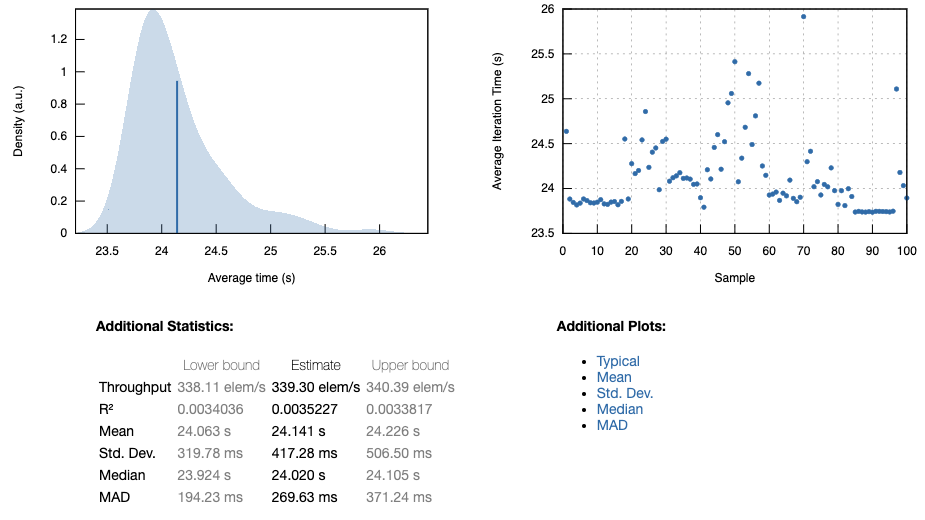
\includegraphics[width=0.9\linewidth]{../assets/html-report-example.png}
  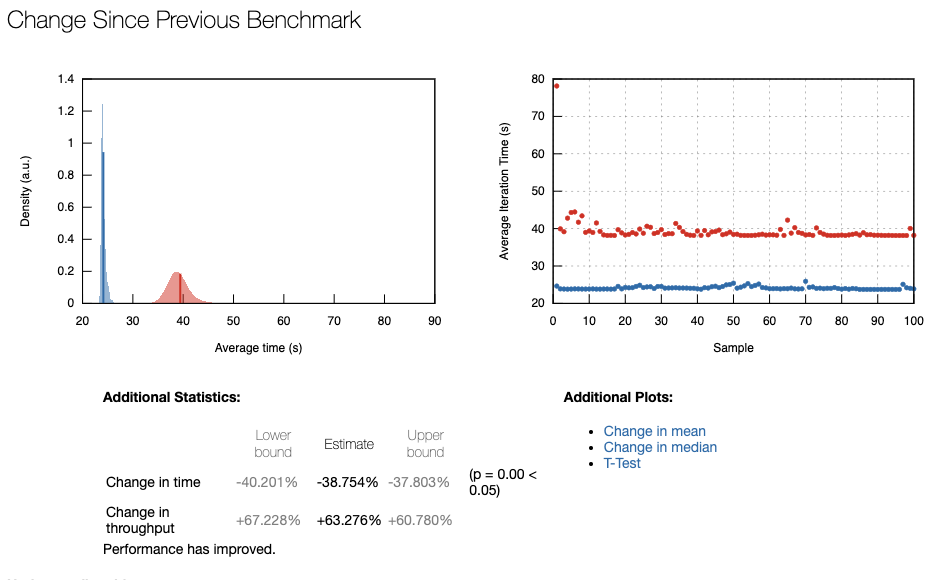
\includegraphics[width=0.9\linewidth]{../assets/performance-change-examplel.png}
  \caption{Example of the HTML report generated by \texttt{criterion}.
  The first image shows an example of the additional statistics that are 
  conveniently provided in the report. The second image shows an example of 
  the performance comparison between two different benchmark runs. If the 
  change in performance falls within a certain threshold, the change is marked as 
  significant.
  }
  \label{fig:criterion-report}
\end{figure}

\subsection{Implementation of Benchmarks}
\label{sec:benchmarks-implementation}
Our goal is to measure the metrics shared earlier and to visualise the data on 
a plot. The main challenge in this task is to ensure that the benchmarks are 
accurate and reliable -- only necessary computation should be measured, and 
appropriate calculations should be used to measure communication size. Hence, 
tests are not suitable for evaluating the validity of our benchmarks, and 
will require a more manual process of accessing the data and ensuring that
the benchmarks are appropriate. In the following subsections, we discuss how 
we implement our benchmarks to achieve these goals. 

\subsubsection{Computation Time} Recall the definition of a $\Sigma$-protocol 
$\Pi = (A, Z, \phi)$. To ensure that we are measuring an accurate estimate 
of the computation time of the prover and verifier, we design and implement the 
benchmarks such that they isolate the execution of the prover algorithms ($A$ and $Z$), 
and the verifier algorithms ($\phi$ and $c \leftarrow \{0,1\}^\kappa$). The key idea 
is that we are implementing a benchmark, hence there is no need to run the 
$\Sigma$-protocol in 
order. We simply precompute the challenge $c$ from the second round of the protocol 
without measuring the time taken to compute it. Next, we execute algorithms $A$ and $Z$ 
in the prover's benchmark, collecting 
data on the computation time. Within this benchmark, 
there may be additional executions that we are not directly interested in but are 
necessary. 
Here we provide an example from the benchmarks of CDS94:


\begin{lstlisting}[language=rust]
  // Precompute challenge
  let challenge = Scalar::random(&mut verifier_rng);

  // Intialize variables to store results from first and third round 
  let mut message_a: Vec<CompressedRistretto> =
      Vec::new();
  let mut message_z: Vec<(usize, Scalar, Scalar)> =
      Vec::new();

  // Benchmarking environment for Prover benchmark
  group.bench_with_input(
      BenchmarkId::new("prover_bench", &proverparams),
      &mut proverparams,
      |b, s| {
          b.iter(|| {
              // Code within these braces are being benchmarked and measured
              // Should have negligible cost 
              let prover_rng = &mut s
                  .prover_rng
                  .clone();
              // First round of protocol
              let (transcripts, commitments) =
                  SelfCompiler94::first(
                      &s.statement,
                      &s.witness,
                      prover_rng,
                  );
              // Third round of protocol
              let proof = SelfCompiler94::third(
                  &s.statement,
                  transcripts,
                  &s.witness,
                  &s.challenge,
                  prover_rng,
              );
              // Should have negligible cost
              message_a = commitments;
              message_z = proof;
          })
      },
  );

  /// ...

  let verifier_rng = &mut ChaCha20Rng::from_entropy();

  // Benchmarking environment for Verifier benchmark
  group.bench_with_input(
      BenchmarkId::new("verifier_bench", &v_params),
      &v_params,
      |b, s| {
          b.iter(|| {
              // Re-execution of second round
              SelfCompiler94::<Schnorr>::second(
                  verifier_rng,
              );
              // Verification algorithm
              SelfCompiler94::verify(
                  &s.statement,
                  &s.message_a,
                  &s.challenge,
                  &s.message_z,
              )
          })
      },
  );
\end{lstlisting}

On line 17 and 36 of the code listing, we indicate (with comments) the blocks 
of code that are necessary and should have negligible cost. These are needed 
to ensure the protocol executes without error and that the output from the 
first and third round can be collected for the verifier's benchmark. Within the 
verifier's benchmark, we re-execute the second round of the protocol (line 53) to ensure
that the verifier's computation time for this round is also measured even though 
the resulting challenge is not used in the verification algorithm.

\subsubsection{Communication Size} 
As mentioned earlier, we use the \texttt{Message} interface to conveniently 
compute the communication size of each benchmark. Once the interface is 
implemented for each required type, measuring the size of the messages 
can be done with a single call to the \texttt{size()} method. 

\begin{lstlisting}[language=rust]
  let mut communication_sizes: Vec<usize> =
        Vec::with_capacity(Q - 1);

  /// ...

  communication_sizes.push(
      message_a.size()
          + message_z.size()
          + challenge.size(),
  );
\end{lstlisting}

To calculate the total communication size, we simply sum the sizes of the 
messages from each round of the protocol. We append this to a vector of 
communication sizes for each number of benchmarks, and use this to 
plot the growth of communication size against the number of clauses.  

\section{General Design Approach for Compiler Components}\label{design:approach}
Our general approach to designing our compiler-related software components is inspired by the 
well-known "SOLID" design principles \cite{martin2000design} of object-oriented programming. 
Crucially, we ensure that our general design approach contributes directly to our core requirements 
of generality and usability. We split our compiler-related software components into two broad categories: 
general interfaces 
and concrete implementations. The general interfaces define the structure of protocols, while the 
concrete implementations are the actual implementations of these interfaces (with possible extensions).

Firstly, we want to ensure that we design our concrete implementations such that 
they \textit{accept general types that implement these interfaces} instead of the concrete 
types directly.
For example, our Stacking Sigmas compiler is designed to 
accept a generic type that requires an implementation of the \texttt{SigmaProtocol} interface and the 
\texttt{EHVzk} interface, instead of accepting the concrete type, which in our case is Schnorr's protocol. 
This allows developers to use the Stacking Sigmas compiler with any $\Sigma$-protocol implementation, as 
long as they implement the relevant interfaces. This also supports our choice to use a microservices architecture and organise our code into separate modules for each component. 
By doing this, modules which define our interfaces should not be importing concrete types; modules 
defining concrete types should only import the interfaces they need to implement and explicitly 
import concrete types that are absolutely necessary. 

We also want to make sure that our interfaces have \textit{a single responsibility} and do not 
encompass too many functionalities. For example, we intentionally segregate the two interfaces 
\texttt{SigmaProtocol} and \texttt{EHVzk}, even though we require both of them to be implemented 
for the Stacking Sigmas compiler. This is so that we do not assume how future users will use 
our interfaces. For the CDS94 compiler, there is the \texttt{HVzk} interface. We know that the 
HVZK property can be thought of as a superset of the EHVZK property because a $\Sigma$-protocol that is 
EHVZK is HVZK, but not necessarily the other way around. With this in mind, we
should not need to implement the simulator as defined in the context of the \texttt{HVzk} interface if 
it is already defined in terms of \texttt{EHVzk}. 
Likewise, a future user may choose to develop a 
\texttt{SigmaProtocol} that has a different requirement for the zero-knowledge property. By 
segregating the interfaces into atomic functionalities, we provide users with more flexibility 
in how they use our interfaces.

Lastly, as mentioned in the testing section \ref{design:testing}, to support static analysis and 
improve the readability of our code, we \textit{design our interfaces to reflect the 
mathematical definitions} of the protocols as much as possible. This facilitates easy 
comparison between our implementations and the mathematical definitions, and helps to 
verify that our implementation is sound. 

% \section{$\Sigma$-protocols}
% \subsection{$\Sigma$-protocols}
\begin{definition}[$\Sigma$-Protocol \cite{StackingSigmas}]
Let $\mathcal R$ be an NP relation. A $\Sigma$-protocol $\Pi = (A, Z, \phi)$ for $\mathcal R$ is a 3-round protocol between a prover algorithm $P$ and a verifier algorithm $V$. The protocol consists of a tuple of probabilistic polynomial time algorithms $(A, Z, \phi)$ with the following interfaces:
\begin{itemize}
    \item $a \leftarrow A(x,w; r^p)$ : Given statement $x$, witness $w \in w(x)$, and prover randomness $r^p$ as input; output the first message $a$ that $P$ sends to $V$ in the first round. 
    \item $c \samplefrom \{0,1\}^\kappa$: $V$ samples a random challenge $c$ and sends it to $P$ in the second round. 
    \item $z \leftarrow Z(x,w,c; r^p)$: Given $x$, $w$, $c$, and $r^p$ as input; output the message $z$ that $P$ sends to $V$ in the third round.
    \item $b \leftarrow \phi(x,a,c,z)$: Given $x$, and the messages in the transcript, output a bit $b \in \{0,1\}$. This algorithm is executed by $V$, and $V$ accepts if $b = 1$.
\end{itemize}
A $\Sigma$-protocol has the following properties:
\begin{enumerate}
    \item \textbf{Completeness.} $\Pi$ is complete if for any $x$, $w \in w(x)$, and any prover randomness $r^p \samplefrom \{0,1\}^\lambda$, the verifier accepts with probability 1. 
    \begin{gather*}
        Pr\left[\phi(x,a,c,z) = 1 \st a \leftarrow A(x,w;r^p); c\samplefrom \{0,1\}^\kappa; z \rightarrow Z(x,w,c;r^p)\right] = 1
    \end{gather*}
    \item \textbf{Special Soundness.} $\Pi$ is said to have special soundness if  there exists a PPT extractor $\mathcal E$, such that given any two transcripts $(a,c,z)$ and $(a,c',z')$ for statement $x$, where $c \ne c'$ and $\phi(x,a,c,z) = \phi(x,a,c',z') = 1$, an element of $w(x)$ can be computed by $\mathcal E$.
    \item \textbf{Special Honest-Verifier Zero-Knowledge (SHVZK).} $\Pi$ is SHVZK if there exists a PPT simulator $\mathcal S$, such that for any $x$, $w$, $(x,w) \in \mathcal R$, the distribution over the output $\mathcal S(1^\lambda, x, c^*)$ is indistinguishable from the distribution over transcripts produced by the interaction between $V$ and $P$ when the challenge is $c^*$.
    \begin{multline*}
        \{(a, z) \mid c^* \samplefrom \{0,1\}^\kappa; (a,z) \leftarrow \mathcal S(1^\lambda,x,c^*)\} 
        \approx_{c^*} \\
        \{(a,z) \mid r^p \samplefrom \{0,1\}^\lambda; a \leftarrow A(x,w;r^p); c^* \samplefrom \{0,1\}^\kappa; z \leftarrow Z(x,w,c^*;r^p)\}
    \end{multline*}
\end{enumerate}
\end{definition}

\begin{definition}[Witness Indistinguishable (WI)]\label{def:wi}
A $\Sigma$-protocol is witness indistinguishable over $\mathcal R$ if for any $V'$, any large enough input $x$, any $w_1,w_2 \in w(x)$, and for any fixed challenge $c^*$, the distribution over transcripts in the form $(a_1, c, z_1)$ and $(a_2,c,z_2)$ are indistinguishable, where $a_i \leftarrow A(x,w_i;r^p)$ and $z_i \leftarrow Z(x,w_i, c^*; r^p)$ for $i \in \{1,2\}$. This means that the prover reveals no information about which are the active clauses. 
\end{definition}

\begin{definition}[Informal definition of Witness Hiding (WH)]\label{def:wh}
For any $x$ that is generated with a certain probability distribution by a generator $\mathcal G$ which outputs pairs $(x,w) \in \mathcal R$, a $\Sigma$-protocol is witness hiding over $\mathcal G$, if it does not help even a cheating verifier to compute a witness for $x$ with non-negligible probability. Refer to \cite{10.1145/100216.100272} for details. WH is a weaker property than general zero-knowledge, as it only asserts that the verifier cannot learn about the witness (not asserting anything about other information). That said, it can replace zero-knowledge in many protocol constructions, as it is in most $\Sigma$-protocols.

\end{definition}



% \section{Schnorr's Protocol}\label{design:schnorr}

\section{Design \& Implementation of Key Components}
In this section, we will highlight the design and implementation 
of important components of our project in their respective subsections.

\subsection{Sigma Protocols}\label{design:sigma}
\subsection{$\Sigma$-protocols}
\begin{definition}[$\Sigma$-Protocol \cite{StackingSigmas}]
Let $\mathcal R$ be an NP relation. A $\Sigma$-protocol $\Pi = (A, Z, \phi)$ for $\mathcal R$ is a 3-round protocol between a prover algorithm $P$ and a verifier algorithm $V$. The protocol consists of a tuple of probabilistic polynomial time algorithms $(A, Z, \phi)$ with the following interfaces:
\begin{itemize}
    \item $a \leftarrow A(x,w; r^p)$ : Given statement $x$, witness $w \in w(x)$, and prover randomness $r^p$ as input; output the first message $a$ that $P$ sends to $V$ in the first round. 
    \item $c \samplefrom \{0,1\}^\kappa$: $V$ samples a random challenge $c$ and sends it to $P$ in the second round. 
    \item $z \leftarrow Z(x,w,c; r^p)$: Given $x$, $w$, $c$, and $r^p$ as input; output the message $z$ that $P$ sends to $V$ in the third round.
    \item $b \leftarrow \phi(x,a,c,z)$: Given $x$, and the messages in the transcript, output a bit $b \in \{0,1\}$. This algorithm is executed by $V$, and $V$ accepts if $b = 1$.
\end{itemize}
A $\Sigma$-protocol has the following properties:
\begin{enumerate}
    \item \textbf{Completeness.} $\Pi$ is complete if for any $x$, $w \in w(x)$, and any prover randomness $r^p \samplefrom \{0,1\}^\lambda$, the verifier accepts with probability 1. 
    \begin{gather*}
        Pr\left[\phi(x,a,c,z) = 1 \st a \leftarrow A(x,w;r^p); c\samplefrom \{0,1\}^\kappa; z \rightarrow Z(x,w,c;r^p)\right] = 1
    \end{gather*}
    \item \textbf{Special Soundness.} $\Pi$ is said to have special soundness if  there exists a PPT extractor $\mathcal E$, such that given any two transcripts $(a,c,z)$ and $(a,c',z')$ for statement $x$, where $c \ne c'$ and $\phi(x,a,c,z) = \phi(x,a,c',z') = 1$, an element of $w(x)$ can be computed by $\mathcal E$.
    \item \textbf{Special Honest-Verifier Zero-Knowledge (SHVZK).} $\Pi$ is SHVZK if there exists a PPT simulator $\mathcal S$, such that for any $x$, $w$, $(x,w) \in \mathcal R$, the distribution over the output $\mathcal S(1^\lambda, x, c^*)$ is indistinguishable from the distribution over transcripts produced by the interaction between $V$ and $P$ when the challenge is $c^*$.
    \begin{multline*}
        \{(a, z) \mid c^* \samplefrom \{0,1\}^\kappa; (a,z) \leftarrow \mathcal S(1^\lambda,x,c^*)\} 
        \approx_{c^*} \\
        \{(a,z) \mid r^p \samplefrom \{0,1\}^\lambda; a \leftarrow A(x,w;r^p); c^* \samplefrom \{0,1\}^\kappa; z \leftarrow Z(x,w,c^*;r^p)\}
    \end{multline*}
\end{enumerate}
\end{definition}

\begin{definition}[Witness Indistinguishable (WI)]\label{def:wi}
A $\Sigma$-protocol is witness indistinguishable over $\mathcal R$ if for any $V'$, any large enough input $x$, any $w_1,w_2 \in w(x)$, and for any fixed challenge $c^*$, the distribution over transcripts in the form $(a_1, c, z_1)$ and $(a_2,c,z_2)$ are indistinguishable, where $a_i \leftarrow A(x,w_i;r^p)$ and $z_i \leftarrow Z(x,w_i, c^*; r^p)$ for $i \in \{1,2\}$. This means that the prover reveals no information about which are the active clauses. 
\end{definition}

\begin{definition}[Informal definition of Witness Hiding (WH)]\label{def:wh}
For any $x$ that is generated with a certain probability distribution by a generator $\mathcal G$ which outputs pairs $(x,w) \in \mathcal R$, a $\Sigma$-protocol is witness hiding over $\mathcal G$, if it does not help even a cheating verifier to compute a witness for $x$ with non-negligible probability. Refer to \cite{10.1145/100216.100272} for details. WH is a weaker property than general zero-knowledge, as it only asserts that the verifier cannot learn about the witness (not asserting anything about other information). That said, it can replace zero-knowledge in many protocol constructions, as it is in most $\Sigma$-protocols.

\end{definition}



\subsection{Shamir's Secret Sharing}\label{design:sss}
For our implementation of Shamir's Secret Sharing, we use Lagrange's interpolating 
polynomial to interpolate the $x$ and $y$ coordinates that correspond to shares. We 
chose to use Lagrange's interpolation formula because it is simple to implement, 
albeit not the most efficient. This trade off is acceptable as the main goal for the project 
is to measure the performance change with respect to the number of clauses, and 
not the pure performance of the compiler. A more efficient implementation is therefore 
not a priority, and can always be implemented in the future if needed. 

Initially, we used an existing library \texttt{vsss-rs} \cite{vsss-rs} as our implementation of 
Shamir's secret sharing scheme. However, we encountered a few issues with this library. Firstly, 
the library does not provide the functionality to complete a qualified shares given the secret 
and an unqualified set of shares. This is not surprising as this is not the main use case for 
a secret sharing scheme like Shamir's. However, this is a necessary feature for our compiler
as we use it to ensure that the prover is unable to arbitrarily select challenges to cheat the 
verifier. We initially tackled this by simply adding the missing functionality to the library, 
in the form of new functions. However, we later found out about the second issue with the library:
its implementation of Lagrange's algorithm is inefficient.

In their implementation, they call the \texttt{invert} 
method in the inner-loop of the algorithm resulting in $n^2$ calls to the function, 
where $n$ is the number of shares. The \texttt{invert} method is required to perform 
division on our group elements, but it is a costly operation. 
This can be avoided, however, by computing the numerator and denominator 
separately and performing the \texttt{invert} function only $n$ times -- outside of the inner-loop. 
The following snippet of code shows the comparison of the two implementations. 

\begin{lstlisting}[language=rust]
  // Inefficient implementation
  for i in 0..n { // outer-loop
    for j in 0..n { // inner-loop
      if i != j
        basis *= (x - x[j]) * (x[i] - x[j]).invert()
      result += basis * y[i]
    }
  }

  // More efficient implementation
  for i in 0..n {
    for j in 0..n {
      if i != j {
        numerator *= x - x[j]
        denominator *= x[i] - x[j]
      }
    }
    result += numerator * denominator.invert() * y[i]
  }
\end{lstlisting}

Due to this issue, we created our own implementation of Shamir's secret sharing scheme. 
We represent a Lagrange polynomial with two fields: 
$x$-coordinates and $y$-coordinates which are both vectors of the same length. 
For a polynomial with degree $d$, the vectors will have length $d$ as well. 

An alternative we considered is to represent the polynomial with a vector of coefficients, 
where the $i$-th element of the vector is the coefficient of the $i$-th degree term. This representation 
is useful in the method for distributing shares given the secret, as we can use Horner's method 
to evaluate the polynomial at a given point efficiently \cite{horner}. However, CDS94 does not 
rely on the secret sharing scheme's functionality for distributing shares, and instead uses
the \textsf{Complete} algorithm (Definition \ref{def:sss-completion}) to complete a qualified set.
For this algorithm, we need to use polynomial interpolation as we are given the secret and an unqualified
set of shares (and equivalently points on the polynomial). 
Therefore, we choose to represent the polynomial in this way because it is more natural for use in 
Lagrange's interpolation formula (Definition \ref{def:lagrange}). 

\subsection{Half-Binding \& Q-Binding}\label{design:qbinding}
Before implementing half-binding and q-bindings, we implement the \texttt{PartialBindingCommScheme} interface 
to model the definition of partially-binding vector commitments provided in Definition \ref{def:comm_scheme}. 
This interface has methods that correspond to each function in the definition: \texttt{setup}, \texttt{gen}, 
\texttt{bind} (equivalent to \textsf{BindCom}), \texttt{equiv}, and \texttt{equivcom}. 
The interface also has a set of generic types to complete the definition of these methods (similar to how 
they function in the \texttt{SigmaProtocol} interface). These generic types are:
\begin{itemize}
  \item \texttt{PublicParams}: public parameters for the commitment scheme. 
  \item \texttt{BindingIndex}: a type that represents the binding index(es) of the commitment. 
  \item \texttt{CommitKey}: a type that represents the commitment key.
  \item \texttt{EquivKey}: a type that represents the equivocation key. 
  \item \texttt{Commitment}: a type that represents the commitment.
  \item \texttt{Randomness}: a type that represents the auxiliary values that are needed for equivocation. 
  \item \texttt{Msg}: a type that represents the vector of messages. 
\end{itemize}

With this interface, we implement \texttt{HalfBinding} and \texttt{QBinding} according to their 
construction in Figure \ref{fig:half-binding} of this report, and Figure 4 of \cite{StackingSigmas} 
respectively. The definition of q-binding is recursive in nature, where the base case is the 
half-binding scheme. In an attempt to improve the usability of our q-binding implementation, we introduce 
some overhead in how we represent the tree of half-bindings. Intuitively, this could simply be a 
recursive data structure, in which every node has two children which continue down until the leaves. 
However, due to Rust's strict type system and our limited experience with the language, we were unable 
to implement this without heavily sacrificing the usability of the interface. 

Instead, we represent the tree as a set of vectors of data types, where each index in the vector represents a 
layer of the tree. We have multiple vectors for each concrete type for the half-binding implementation of the 
\texttt{PartialBindingCommScheme} interface. While this introduces some overhead as the vector must be 
traversed if we want to copy the data, it allows us to implement the interface in a way that has good 
usability and is still easy to understand. We hypothesize that this is the main reason our implementation of 
Stacking Sigmas is slower than Hall-Andersen's implementation \cite{MHAStackSig}. This will be discussed in 
Chapter \ref{sec:evaluation} in more detail. 

Lastly, we would like to point out a flaw in our current implementation of the q-binding scheme. Currently, there is no data for the disjunction of 2 clauses for Stacking Sigmas (refer to Table \ref{tab:comm-size}) because of this flaw. This is because we did not define the base case of our recursion correctly, which should be 
a simple half-binding scheme. Instead, we initialise the case for 2 clauses with a q-binding scheme 
that makes use of two half-binding schemes, resulting in 4 clauses. This was revealed after inspecting the results of the benchmarks and realising equal communication sizes for 2 clauses and 4 clauses. We are currently working on a fix for this bug. As a temporary measure, we change the minimum number of clauses to 4 instead of 2 to avoid any errors.

\subsection{\texttt{HVzk} \& \texttt{EHVzk} Interface}
These two interfaces encompass the honest-verifier and extended honest-verifier zero-knowledge 
property respectively, which means that the only required method for these two interfaces 
is a simulator method (Definition \ref{def:sigma}) for the concrete $\Sigma$-protocol that 
implements this interface. As mentioned in the section on the general approach to design, 
we split this interface from the \texttt{SigmaProtocol} interface to adhere to the 
"single responsibility" principle in "SOLID" design \cite{martin2000design}. We provide 
code-snippets of these two interface in Appendix \ref{code:hvzk}.

\subsection{CDS94 Compiler}\label{design:cds94}
We implement the CDS94 compiler for disjunctions over the same $\Sigma$-protocol. This means we are concerned 
with many instances of the same $\Sigma$-protocol, even though it is possible to use CDS94 to compile 
disjunctions over different $\Sigma$-protocols. We do this to simplify our implementation and to focus on the 
most basic implementation of the CDS94 compiler. The disjunctions that this compiler supports are $d$-out-of-$n$
disjunctions, where $d$ is the minimum number of active clauses, and $n$ is the total number of clauses.
At a high level, the design of the CDS94 compiler is not complex and simply follows the construction provided 
in Protocol \ref{prot:cds-compiler}. That said, we make certain design decisions that are worth highlighting.

Firstly, we cannot only implement the \texttt{SigmaProtocol} interface for the underlying $\Sigma$-protocol
that we want to use with the CDS94 compiler.
This is because the CDS94 compiler requires further restrictions on the generic 
types that is used during a concrete implementation. Notably, Shamir's secret sharing scheme requires that 
the shares passed to it have $x$ and $y$ coordinates that are field elements. This means we need to 
provide a way to map the generic \texttt{Challenge} type (from \texttt{SigmaProtocol} interface) to a 
type that implements the \texttt{PrimeField} interface from the \texttt{group} library (Section \ref{sec:libraries}).
For Schnorr's protocol, this is not a theoretical issue because the challenges that are used are field elements
and can be used directly with Shamir's secret sharing. However, in practice, the \texttt{Scalar} type from the
\texttt{curve25519-dalek} library does not implement the required interface. 

An alternative is to directly require that the \texttt{Challenge}
type parameter in the \texttt{SigmaProtocol} interface to implement the \texttt{PrimeField} interface. However,
this is arguably more restrictive than necessary. This is because we may have existing implementations of a 
$\Sigma$-protocol that does not use a challenge that is a field element, but we still want to use it with the
CDS94 compiler. In this case, we can simply define a mapping function that maps the challenge to a field element
and use it with Shamir's secret sharing. 
Hence, to capture this relationship, we introduce the \texttt{Shareable} interface.

\paragraph{\texttt{Shareable}.} A simple interface to ensure type-level compatibility between 
the generic types used in the CDS94 compiler and the generic types used in Shamir's secret sharing scheme.
This interface is defined as follows: 
\begin{lstlisting}[language=rust]
  pub trait Shareable: Clone + Default {
      type F: PrimeField;
      // Map the type to a prime field element
      fn share(&self) -> Self::F;
      // Derive the instance of the type from a field element
      fn derive(elem: Self::F) -> Self;
      // Convert field element into usize
      fn to_usize(elem: Self::F) -> usize;
  } 
\end{lstlisting}
\begin{itemize}
  \item The concrete type that implements this interface can be any type that also implements the \texttt{Clone} and
  \texttt{Default} traits. 
  \item The \texttt{F} type parameter is a type that implements the \texttt{PrimeField}
  interface from the \texttt{group} library. 
  \item The \texttt{share} method is a function that maps the generic
  type to the \texttt{F} type parameter.
\end{itemize}

This allows developers to implement the \texttt{Shareable} interface for any type that they want to use in the
CDS94 compiler, as long as it is possible to define a mapping function from the chosen type to one that 
implements the \texttt{PrimeField} interface. 
For example, in the case of Schnorr's protocol, the \texttt{Challenge} type is a \texttt{Scalar}
from the \texttt{curve25519-dalek} library. This type does not implement the \texttt{PrimeField} interface, but
we can implement the \texttt{Shareable} interface for it as follows:
\begin{lstlisting}[language=rust]
  impl Shareable for Scalar {
      type F = WrappedScalar;
      // ...
  }
\end{lstlisting}

where \texttt{WrappedScalar} is a wrapper type that implements the \texttt{PrimeField} interface for the 
\texttt{Scalar} type\footnote{We omit the implementation of the methods as they are specific to the 
\texttt{WrappedScalar} type and are not relevant to the discussion here.}.


\paragraph{\texttt{Composable}.} With the \texttt{Shareable} interface, we can now implement the \texttt{Composable}
interface for the base $\Sigma$-protocol to be compiled by CDS94. This interface is defined as follows:

\begin{lstlisting}[language=rust]
  pub trait Composable: SigmaProtocol<Challenge: Shareable> + HVzk {}
\end{lstlisting}

This is a simple interface that enforces the requirement for the base protocol to implement 
the \texttt{SigmaProtocol} interface, with a \texttt{Challenge} type implementing the \texttt{Shareable} 
interface, and to also implement the \texttt{HVzk} interface.

\paragraph{\texttt{CDS94}.} With the \texttt{Shareable} and \texttt{Composable} interfaces, we can now implement
the \texttt{CDS94} compiler. We require that the base $\Sigma$-protocol be compiled implements the
\texttt{Composable} interface. Let this generic type corresponding to the base $\Sigma$-protocol be 
denoted by \texttt{S}. With \texttt{S}, we can define the generic types associated with the \texttt{SigmaProtocol} interface 
for CDS94:

\begin{itemize}
  \item \texttt{Statement}: \texttt{Statement94<S>} -- a type that contains public information 
  for the disjunctive proof: the number of clauses, the threshold, and the statement for each 
  clause of type \texttt{S}.
  \item \texttt{Witness}: \texttt{Witness94<S>} -- a type containing the private information for the 
  disjunctive proof: the witnesses for each clause, and the indexes of the active clauses 
  \item \texttt{MessageA}: \texttt{Vec<S::MessageA>} -- a vector of messages corresponding to the 
  first message in the $\Sigma$-protocol \texttt{S} for each clause.
  \item \texttt{Challenge}: \texttt{S::Challenge} -- the challenge type for the base $\Sigma$-protocol \texttt{S}.
  \item \texttt{MessageZ}: \texttt{Vec<(usize, S::Challenge, S::MessageZ)>} -- A vector of tuples containing 
  the index of the clause, the challenge corresponding to the clause, and the third message \texttt{z} 
  of that clause.
  \item \texttt{State}: \texttt{State94<S>} -- the relevant information generated from the first round
  of the disjunctive protocol that should be private to the Prover. This 
  contains the state of each instance of the base $\Sigma$-protocol (in each active clause), 
  the simulated challenge and 
  third messages $c_i$ and $z_i$ respectively for each inactive clause. 
\end{itemize}

With these generic types, we implement the methods according to the construction in Protocol \ref{prot:cds-compiler}.
Interested readers can compare how our implementation models the construction by referring to the source code 
in Appendix \ref{code:cds}.

\subsection{Stacking Sigmas Compiler}\label{design:stacking}
Similarly to CDS94, we implement the self-stacking compiler for Stacking Sigmas where 
we are concerned with disjunctions of the same $\Sigma$-protocol. An important distinction between 
the two compilers is that the Stacking Sigmas compiler is a 1-out-of-$n$ compiler, where $n$ is the
number of $\Sigma$-protocols in the disjunction. Goel \emph{et al} does include a brief outline of 
how a $d$-out-of-$n$ compiler may be constructed in Section 9 of \cite{StackingSigmas}, but we deem 
this out of scope for the project. 

In our implementation, we compile Schnorr's protocol, using the 
compiler protocol together with the q-binding scheme (Definition \ref{sec:qbinding}).
Overall, the methods associated with the \texttt{SigmaProtocol} library that we implement for the 
\texttt{SelfStacker} class follow the construction in Protocol \ref{prot:stacksig-compiler} closely. 
More interestingly, the generic types and interfaces involved are worth discussing in detail.

\texttt{\texttt{Message}.} This interface is useful in the Stacking Sigmas compiler 
for hashing the messages provided to the partial-binding vector commitments. This is 
an important efficiency requirement outlined in Definition \ref{def:comm_scheme}. 
With the \texttt{Message} interface, we require messages to the partial-binding vector
commitments to be writable to a buffer, which can then be hashed. Additionally, this 
provides a convenient interface for our benchmarks to measure the size of our messages. 

\begin{lstlisting}[language=rust]
  pub trait Message: Debug + Default + Clone {
      fn write<W: Write>(&self, writer: &mut W)
      where
          Self: Sized;

      fn size(&self) -> usize {
          let mut v: Vec<u8> = Vec::new();
          self.write(&mut v);
          v.len()
      }
  }  
\end{lstlisting}

Observing this code-snippet, we can see that once we are able to use the \texttt{write} 
method to write bits of the message to a buffer, we can trivially obtain the size of 
the message by writing it to a vector and then obtaining the length of the vector.

As mentioned earlier, this interface was implemented by Hall-Andersen in 
\cite{MHAStackSig}, and we have extended it slightly. In particular, we further require types 
that implement the \texttt{Message} interface to also implement the \texttt{Default} interface. 
This is a useful addition 
because we can use this to create a default instance of the message type when we are 
using the q-binding scheme. Recall that this scheme requires the "0" message for the 
\textsf{EquivCom}, \textsf{Equiv}, and \textsf{BindCom} methods.

\paragraph{\texttt{Stackable}.} This interface is similar to the \texttt{Composable}
interface in the CDS94 compiler. This interface models a $\Sigma$-protocol that is stackable 
by the Stacking Sigmas compiler.

\begin{lstlisting}[language=rust]
  pub trait Stackable: SigmaProtocol<MessageA: Message, MessageZ: Message> + EHVzk {}
\end{lstlisting}

From its definition, we can see that the main requirements are the \texttt{SigmaProtocol} 
interface and the \texttt{EHVzk} interface, which corresponds correctly to the definition 
of a stackable $\Sigma$-protocol in Definition \ref{def:stackable}. 

\paragraph{\texttt{StackingSigmas}.} The concrete class of the Stacking 
Sigmas' "Self-Stacking" compiler is the \texttt{Self\-Stacker<S>} class, where \texttt{S} 
is a class that implements the \texttt{Stackable} interface. The generic types that 
are associated with this class are:
\begin{itemize}
  \item \texttt{Statement}: \texttt{StackedStatement<S>} -- a type that contains public information 
  for the disjunctive proof: the public parameters $pp$ for the q-binding scheme, 
  the height of the commitment tree, the number of clauses in total, and the 
  vector of messages which correspond to the statement 
  for each clause of type \texttt{S} .
  \item \texttt{Witness}: \texttt{StackedWitness<S::Witness>} -- a type containing the 
  private information for the disjunctive proof: the witnesses for the active clause (only 1), 
  and the index of the active clause.
  \item \texttt{MessageA}: \texttt{StackedA} -- the first message of the Stacking Sigmas 
  protocol (Definition \ref{prot:stacksig-compiler}). This is a 2-tuple, containing 
  the commitment key and the commitment. 
  \item \texttt{Challenge}: \texttt{S::Challenge} -- the challenge type for the base $\Sigma$-protocol \texttt{S}.
  \item \texttt{MessageZ}: \texttt{StackedZ<S>} -- the third message of the Stacking 
  Sigmas protocol containing: the commitment key, the third message ($z$) of the 
  underlying $\Sigma$-protocol, and the auxiliary value needed for the q-binding scheme.
  \item \texttt{State}: \texttt{State94<S>} -- the relevant information generated from the first round
  of the disjunctive protocol that should be private to the Prover. This 
  contains the state of the underlying $\Sigma$-protocol, the first message of the 
  underlying $\Sigma$-protocol, the initial messages given to the q-binding scheme 
  in the first round of the Stacking Sigmas protocol, the commitment key, the equivocation 
  key, and the auxiliary value for the q-binding scheme.
\end{itemize}

With these generic types, we implement the methods for the \texttt{SelfStacker} class
according to Protocol \ref{prot:stacksig-compiler}. Refer to Appendix \ref{code:stacksig} 
for the implementation.





% \section{CDS94 Compiler}\label{design:cds94}

% \section{Half-Binding \& Q-Binding}\label{design:qbinding}

% \section{Self-Stacking Compiler}\label{design:stacking}
